\documentclass[11pt, oneside]{article}   	% use "amsart" instead of "article" for AMSLaTeX format

\usepackage{array}
\setlength{\parindent}{4em}
\setlength{\parskip}{1em}
\renewcommand{\baselinestretch}{1.5}

\usepackage{geometry}                		% See geometry.pdf to learn the layout options. There are lots.
\geometry{letterpaper}                   		% ... or a4paper or a5paper or ... 
%\geometry{landscape}                		% Activate for rotated page geometry
%\usepackage[parfill]{parskip}    		% Activate to begin paragraphs with an empty line rather than an indent
\usepackage{graphicx}				% Use pdf, png, jpg, or eps§ with pdflatex; use eps in DVI mode
								% TeX will automatically convert eps --> pdf in pdflatex		
\usepackage{amssymb}
\usepackage{listings}
\usepackage{tikz-qtree}
\usepackage[document]{ragged2e}
\usepackage{graphicx}				% Use pdf, png, jpg, or eps§ with pdflatex; use eps in DVI mode	
\usepackage{amsmath}



\title{COMP9417 - Assignment 2}
\author{Avinash K. Gupta, Yuyang Shu, Maria Oei}
%\date{}							% Activate to display a given date or no date

\begin{document}
\maketitle

\justify
\section{Introduction}
\section{Introduction}
\par With over 100 millions of monthly visitor in Quora, it is inevitable that many people are asking similar questions. This has become an issue as user has to read through responses to many questions in order to find the best answer. The aim of this project is to implement algorithms to identify 2 similar questions which can help Quora in improving user experience by finding high quality answers to questions.

\par The 2 approaches used in this project were perceptron learning and LSTM. In the perceptron learning, we used 3 inputs which measured semantic similarity, word order and word overlaps between 2 sentences. In LSTM, we provide word-embedding vectors supplemented with synonymic information and calculates the manhattan distance between the vectors.

\par We will see that for our case the performance of the 2 models were quite similar. However, there are other research done on LSTM where it has been shown that LSTM has the potential to performs well with enough training and with careful selection of initial weight.


\section{Methodology}
\section{Methodology}
In this project, we used WordNet as the main lexical database. Using WordNet, we were able to extract the part-of-speech tags for a word as well as their synset (synonym set). This played an important role in determining the similarity of 2 words.

\subsection{Data Preparation}
The training data provided contained pairs of questions and indicators to determine if the two questions were similar. In the first model, each sentence was tokenized into list of words and each word was stemmed to their base form. As a word could be associated to multiple synsets, we used Lesk algorithm to choose the correct synset given the context of the sentence. In Lesk algorithm, for each possible synset we collected its hypernyms and hyponyms into  a list. We then counted the number of common words from this list with the remaining words in the sentence. The synset with the highest number of overlap will then be chosen to be the best synset for the word. Once this was done, stop words were removed and the tokens were sent to a function which computed the semantic similarity and word order score of the 2 sentences. Please see appendix for more details on how to calculate these measures. 

For the LSTM model, the input for the neural network is the individual word in the sentences. One way to translate words into features that could be accepted by machines is to use one hot encoding, with which each word would be translated into a boolean vector whose length equals the size of the vocabulary. Due to the large size of English vocabulary, dimension reduction methods need to be applied on the resulted boolean vector. 

A better way to represent words would be to project each word into a real valued vector space. This method is invented by Google and has proven success in literatures. Hence, we adopt this method to preprocess our data. After preprocessing, each question would be represented by a list of vectors, each of which representing the original word.

\subsection{Training \& Model Selection}
To train the data we used the measures from the above procedure as the features. The original model proposed in (Li et al. 2016) was designed to map each feature to be between 0 and 1. There was also a constraint put on the weights to ensure that the sum of the weights was 1. We tried perceptron learning in order to automate the learning process for the weight. The perceptron initialized the weights to be small random variable with 0.1 learning rate and 1000 iteration. However, we found that the parameters did not converge even after 2000 iterations. By plotting the data against the semantic similarity score and the word order score, it appeared that the data is not linearly separable thus a non-linear model was required. 

Although the bag of words with Naive Bayes seems to be an ideal choice for this problem, because we are dealing with short sentences, these models will not work well as they rely on pure statistics of word frequencies.
After some research, we decided that the LSTM recursive neural network would be the best model for measuring semantic similarity. This model provided a similarity measure afterwhich we could learn the optimal decision boundary to decide whether or not the question pair was a duplicate.
\subsection{Method 1 : Perceptron}

The first model was a a simple perceptron with 2 inputs which were based on [insert reference to paper here]. The inputs chosen measured the semantic similarity and the word order information of the 2 sentences. For each sentences pair in the dataset, both semantic similarity and word order score were calculated. The perceptron weights were then trained based on these measures.

\subsubsection{Words Similarity}
A \textbf{path length} between 2 words is the number of synsets we visit from one word to another. For example, in the figure below, to get from boy to girl we have to visit boy - male - person - female - girl. Therefore, the path length of 'boy' and 'girl' is 4. 'Person' is called the subsumer of 'boy' and 'girl'. If there are more than 1 path, we will consider the shortest path and the corresponding subsumer is called the \textbf{lowest subsumer}.

\begin{center}
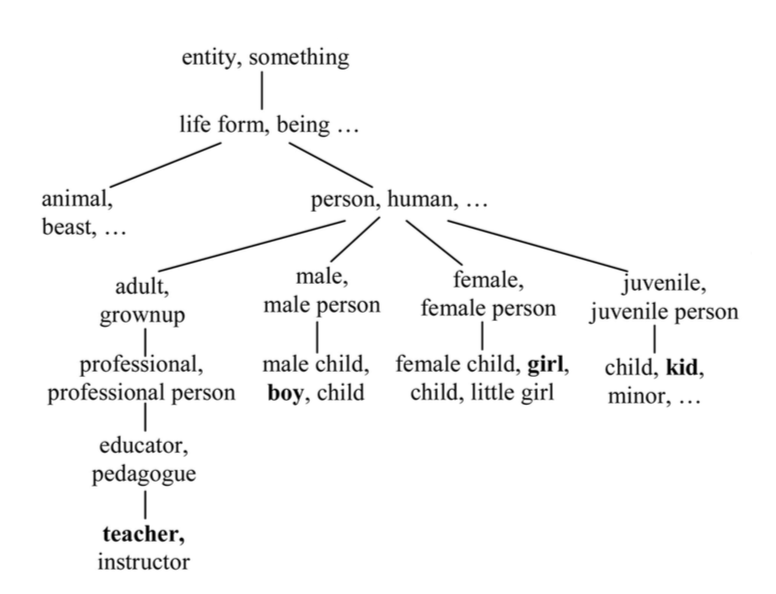
\includegraphics[scale=0.7]{Synset_tree}
\end{center}

Let $l$ denote the shortest path and $h$ denote the depth of the lowest subsumer. The similarity between 2 words $w_1$ and $w_2$ is therefore measured by 
\begin{equation*}
s(w_1, w_2) = f_1(l) f_2(h)
\end{equation*}
where $\alpha, \beta \in [0,1]$ and 
\begin{align*}
	f_1(l)		&= e^{-\alpha l} \\
	f_2(h)	&= \frac{e^{\beta h} - e^{-\beta h}}{e^{\beta h} + e^{-\beta h}} \\
\end{align*}

\subsubsection{Semantic Similarity}
Let $T_1$ and $T_2$ be the 2 sentences and T is a set of distinct words in T1 and T2. For each sentence, we will calculate the vector $s_k$ which the same length as T. For each word $w_i$ in T, we assign 1 to the corresponding element in $s_k$ if $w_i$ is in $T_k$ and $\mu_i$ otherwise. $\mu_i$ is the similarity score between $w_i$ and the most similar word in $T_k$ calculated based on the similarity score above. Once $s_1$ and $s_2$ are calculated, the overall semantic similarity score is calculated by 
\begin{equation*}
	S_s = \frac{s_1. s_2}{||s_1||.||s2||}
\end{equation*}

\subsubsection{Word Order}
Similar to the semantic similarity, we calculate the vectors $r_1$ and $r_2$ for each of the sentences. For each word $w_i$ in T, we set the $i^{th}$ element in $r_k$ to equal to the position of $w_i$ in $T_k$. If $w_i$ is not in $T_k$ then we find the most similar word in $T_k$ and assign the position of that word instead.

For both word order and semantic similarity measure, we define a threshold for the case where $w_i$ is not in $T_k$. If the similarity score between $w_i$ and the most similar word is less than the threshold, 0 will be assigned instead.

For the word order, the overall score is calculated by 
\begin{equation*}
	S_r = 1 - \frac{||r_1 - r_2||}{||r_1 + r_2||}
\end{equation*}



\pagebreak
\subsection{Method 2 : LSTM - RNN}
\subsection{LSTM - RNN}
\subsubsection{Overview}
\par In this approach, we present  siamese adaption of Long Short-Term Memory(LSTM) network for labeled data contains pairs of variable-length sequences. This model is used to get the semantic similairty between the sentences using complex neural network. For this applications, we provide word-embedding vectors supplemented with synonymic information to the LSTMs, which use a fixed size vector to convert the syntactic meaning of the sentence. 

\subsubsection{Model}
\par It's a supervised learning model, where each data consists of pair of sequences 
$(x_1^{(a)},...,x_{n_a}^{(a)})$, $(x_1^{(b)},...,x_{n_b}^{(b)})$ of fixed size vectors along with a single label y(human labeled) for the pair. Note that sequences may be differenent length. These data will be pass to the model with a purpose of learning the semantics. 
 \begin{figure}[h]
    \centering
    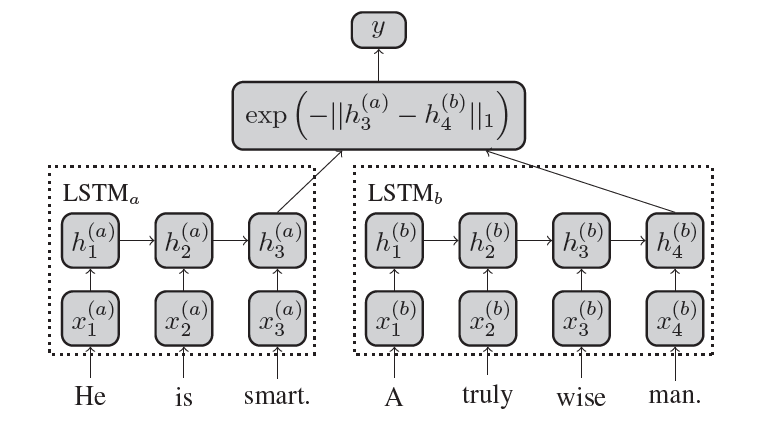
\includegraphics[width=.75\textwidth]{lstm_image}
    \caption{lstm architecture}
\end{figure}
In the above diagram, there are two networks $LSTM_a$ and $LSTM_b$, each of them process a sentence in a given pair and predict whether  $LSTM_a=LSTM_b$ based on the similarity between the vectors. In each LSTM, the word vector is employ to the hidden layer and calculation is done and output is passed to the next hidden layer to remember the previous context and so on.
 \begin{figure}[h]
    \centering
    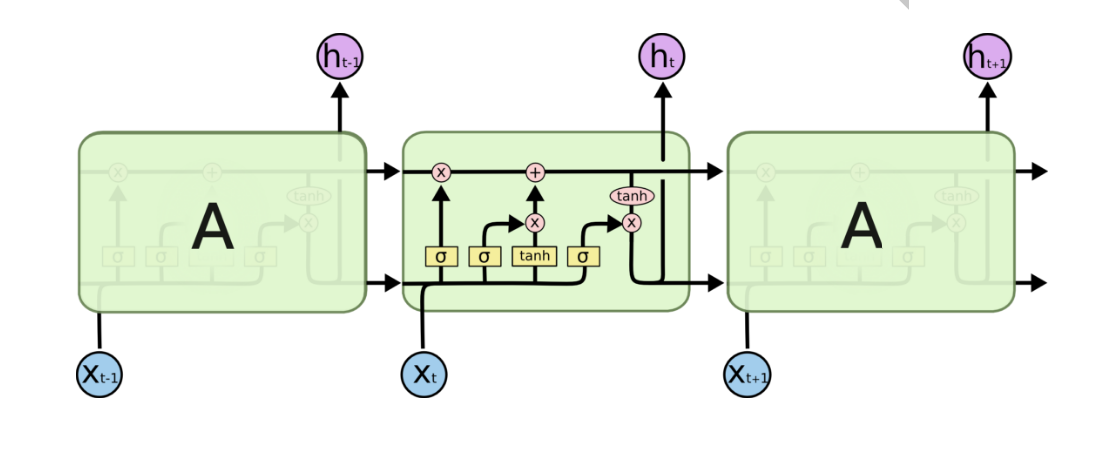
\includegraphics[width=.85\textwidth]{hidden_layer}
    \caption{repeating module of hidden layer}
\end{figure}
In above figure, the hidden layer which is core part of our neural network. It performs operation listed below on each word vector.
\begin{itemize}
\item The first sigmoid function is used to decide which information to keep and what to ignore
$$f_t=sigmoid(W_ix_t + U_ih_{t-1}+b_i)$$
\item Now it's time to update the old cell state into new cell state. The last step already decided what to do, in this step we just actually need to do it.
$$i_t=sigmoid(W_fx_t + U_fh_{t-1}+b_f)$$
$$c_t^`=\tanh(W_cx_t + U_ch_{t-1}+b_c)$$
\item In this step, we will multiply old state $c_{t-1}$ with $f_t$ to forget things we decided to forget earlier. Then we add to new candidate values
$$c_t=i_t \odot c_t^` + f_t \odot c_{t-1}$$
\item Final step defines what we actually need to output based on out filtered cell state and then $\tanh$(used to push values between -1 and 1) and multiply with sigmoid function to decide the parts we need to output.
$$o_t=sigmoid(W_ox_t + U_oh_{t-1}+b_o)$$
$$h_t=o_t \odot \tanh(c_t)$$
\end{itemize}

Above process are carried by both the LSTM and emploed to the Similarity Function given below, which calculates the Manhattan differnece between the ouputs.
$$g(h_{T_a}^{(a)},h_{T_b}^{(b)})=\exp(\textendash \parallel h_{T_a}^{(a)} \textendash h_{T_b}^{(b)}\parallel_1) \in [0,1]. $$

\section{Result \& Discussion}
%\section{Result \& Discussion}


\subsection{Challenges}
The first challenge we face is, what should our vocabulary be, if we were to project the vocabulary into a vector space ourselves. One way is to use all words in the training set, but since embedding requires huge amounts of data to be accurate, this can't work well. Another way could be, to retrieve all questions on Quora, and use the words in all those questions as the vocabulary. The problem of this method is, we would actually be peeking into the testing set, since inevitably the testing set would be from Quora. A third method would be, to use some third party source to construct the vocabulary and the corresponding word vectors.

We believe the third method is the best, and hence we use the Google News vectors (https://drive.google.com/file/d/0B7XkCwpI5KDYNlNUTTlSS21pQmM) as our embedding.

The second challenge is that, due to the computational complexity and hardware dependencies of the model, specifically the requirements of the theano package, we were not able to replicate the training of the LSTM model ourselves before the deadline of the project. Instead, we used a pre-trained model to do the prediction, namely the Siaseme LSTM (https://github.com/aditya1503/Siamese-LSTM) model trained based on the sentences involving compositional knowledge dataset (Marelli et al 2014) as a proxy. We feed the question pairs into the Siaseme model, and it would produce the similarity measure between them. We then run a simple test to find the threshold beyond which we should predict duplicate.

If we were to train the LSTM RNN ourselves, we would feed it with our labelled data, in the form of (question 1, question2, label) where label is a boolean indicating whether the two questions are duplicate or not, and the test data would be in the form of (question 1, question2). This way, the model performance would be much better.

\subsection{Conclusion}
\subsection{Limitation \& Improvement}



\end{document}  